% !TeX spellcheck = de_DE
\clearpage

\newboolean{includeWiki}
\setboolean{includeWiki}{false}


\section{\ExercisePrefixEmbeddedC WSN---Wide Sensor Network\optional}
\newcommand{\toolWSN}{\textsc{WSN}\xspace}

\optionaltextboxC

Ein \toolWSN (Wide Sensor Network) ist ein Netzwerk aus verteilten Sensorknoten. Ziel dieser Aufgabe ist es, das Mikrocontrollerboard um weiteren Mikrocontroller mit WiFi-Schnittstelle zu erweitern, sodass mehrere Boards über ein drahtloses Netzwerk (WLAN) kommunizieren können. Dieses Netzwerk soll verwendet werden, um gemessene Sensordaten an eine zentralen Server-Anwendung zu senden.

Als Erweiterungsmodul nutzen wir das ESP-12E Modul. Dieses wird mit einer modifizierten Version der \href{https://github.com/martin-ger/esp_wifi_repeater}{esp\_wifi\_repeater-Firmware} betrieben. Die Kommunikation zwischen unserem Mikrocontroller und dem ESP-Board wird über UART realisiert. 

\begin{enumerate}
	\item Unser Mikrocontrollerboard besitzt insgesamt 12 serielle Schnittstellen. In dieser Aufgabe verwenden wir die Schnittstelle UART3, welche über den Multicon-Pinheader (rote Markierung) verfügbar ist. 
	
	%[Grafiken]
		
	\begin{minipage}{.4\textwidth}
		\centering
		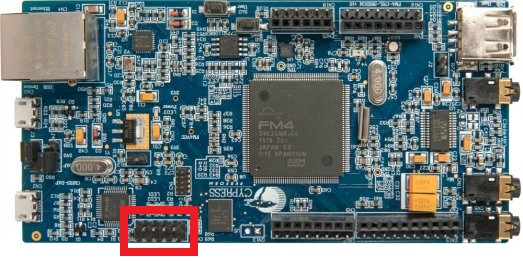
\includegraphics[width=\textwidth]{./05_c/figures/s6e2cc.jpg}
		%\captionof{figure}{Position des Pinheaders auf dem Board}
		%\label{fig:s6e2cc}
	\end{minipage}
	\begin{minipage}{.5\textwidth}		
		\centering
		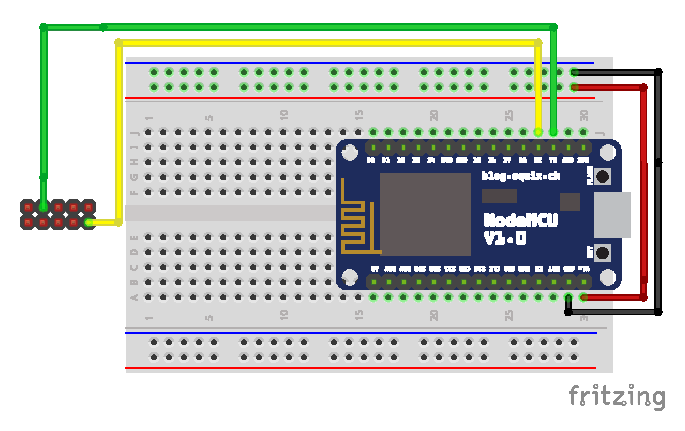
\includegraphics[width=\textwidth]{./05_c/figures/wsnWiring_Steckplatine.pdf}
		%\captionof{figure}{Verkabelung der Platinen}
		%\label{fig:wiring}
	\end{minipage}

	Zuerst muss das ESP-Board wie in den beiden Abbildungen zu sehen angeschlossen werden. Dazu sind 4 Leitungen nötig: Masse (GND), Versorgungsspannung (Vcc), von Tx (Transmit) am Cypress-Board zu Rx (Receive) am ESP-Modul und vice versa.

	\item Um nun Daten in Form von Zeichenketten zu übertragen, muss zuerst die UART-Schnittstelle initialisiert werden. Dazu reicht es, den Header \lstinline|uart_multicon.h| einzubinden und die Funktion \lstinline|cpp_initUart3Baud(115200)| aufzurufen. \lstinline|115200| ist die Baudrate mit der die Schnittstelle arbeiten muss.
	
	Zum Übertragen von ganzen Zeichenketten, ist es hilfreich zunächst eine Funktion zu implementieren, welche ein einzelnes Zeichen als Parameter entgegennimmt und überträgt (\zB \lstinline|void writeCharUart3(char c)|). In dieser Funktion muss gewartet werden, solange der Aufruf \lstinline|Mfs_Uart_GetStatus(\&UART3, UartTxEmpty)| nicht \lstinline|TRUE| ergibt. \lstinline|TRUE| und \lstinline|FALSE| sind in diesem Fall Makros der Treiberbibliothek, und müssen daher genau so verwendet werden. Liefert der \lstinline|Mfs_Uart_GetStatus|- Aufruf \lstinline|FALSE| zurück, ist die Schnittstelle bereit um ein einzelnes Zeichen mit dem Aufruf von \lstinline|Mfs_Uart_SendData(&UART3, 'c')| zu versenden.
	
	\item Implementiere nun noch eine Funktion die einen nullterminierten C-String entgegennimmt und durch wiederholte Aufrufe von \lstinline|writeCharUart(char c)| versendet.
	
	Teste deine Funktion, indem du ihr einen Text (\zB \lstinline|"mqtt_pub /Hello World!\r\n"|) übergibst. \lstinline|\r\n| markiert das Ende des Befehls. Auf der Serveranwendung sollte deine Nachricht nun ankommen.
	
	\item Erweitere nun dein Board um einen Sensor, und sende den gemessenen Sensorwert an die Zentrale Serveranwendung. Sende dazu den Befehl \lstinline|"mqtt_wsn <Sensorwert>\r\n"|.
\end{enumerate}	

\ifthenelse{\boolean{includeWiki}}{

		\newpage
		\renewcommand{\thesubsection}{}
		\renewcommand{\thesubsubsection}{}
		\subsection{Mini-Wiki}
		
		In diesem Abschnitt sollen die anderen Teile des WSN näher eräutert, und auf deren Funktion eingegangen werden. 
		
		\subsubsection{MQTT} 
		Message Queuing Telemetry Transport (MQTT) ist ein Client-Server-Kommunikationsprotokoll, das auf dem Publish-Subscribe-Muster beruht. Weite Verbreitung hat MQTT in IoT-Szenarien, z.B. bei der Übermittlung von Sensordaten. Ein zentraler Server (Broker) verwaltet hierbei alle Nachrichten in einer hierarchischen Topic-Struktur.  Clients können sich mit dem Broker verbinden und entweder Daten auf einem Topic veröffentlichen (publish), oder ein Topic abonnieren (subscribe), was den Broker dazu veranlasst alle eingehenden Nachrichten eines Topics an den Clienten weiterzuleiten.
			
		Die einzelnen Hierarchiestufen eines Topics werden dabei durch Schrägstriche ('/') voneinander getrennt. Durch Nutzung von Wildcards können nicht nur konkrete Topics, sondern auch Bereiche von Topics abonniert werden. '+' steht dabei als Wildcard für alle Topics der jeweiligen Hierarchiestufe, '\#' schließt auch alle darunterliegenden Topics mit ein, und muss daher immer am Ende der Topic-Definition stehen.
		
		\subsubsection{UART} 
		Universal-Asynchronous-Receiver-Transmitter (UART) ist eine einfache elektronische Schnittstelle zur seriellen Datenübertragung. Es wird häufig verwendet um Daten zwischen Mikrocontrollern und anderen elektronischen Komponenten (e.g. andere Mikrocontroller, Sensoren) auszutauschen.
		
		\subsubsection{WiFi}
		Grundsätzlich gibt es zwei Typen von WiFi-Schnittstellen: Station und Access Point. Eine Station ist in diesem Kontext ein Gerät, welches ein WiFi-Netz aufspannt, eine Station wählt sich in das Netz eines Access-Points ein.
		Die meisten Geräte besitzen nur eine Schnittstelle, und sind somit Station \emph{oder} Access Point.
		
		\subsubsection{ESP12-E}
		Das ESP-12E ist ein Mikrocontrollerboard welches den weit verbreiteten ESP8266 für die Benutzung auf einem Steckbrett optimiert. So stellt es \zB einen Micro-USB Anschluss und zwei Buttons bereit, und führt die Anschlüsse des Mikrocontrollers zum einfacheren Zugriff zu angelöteten Pins.
		
		Im Kontext dieses Projekts ist es wichtig zu erwähnen, dass der ESP8266 in einem kombinierten Modus gleichzeitig als Station und Access Point betrieben werden kann.
		
		\subsubsection{esp\_wifi\_repeater}
		Die esp\_wifi\_repeater-Firmware implementiert die Funktionalität eines NAT-Routers auf dem ESP12E-Board. Da der dort verwendete Mikrocontroller gleichzeitig Station und Access-Point sein kann, ist es möglich ihn als Repeater zu verwenden. Die Firmware bietet im sogenannten \emph{Automesh-Mode} die Möglichkeit der selbstständigen Konfiguration. Im Automesh-Mode werden dem Mikrocontroller nur die SSID und das Passwort des zu Erweiternden Netzwerkes angegeben.
		
		Die Konfigurationsparameter werden dabei auf dem Flashspeicher des Chip geschrieben. Bootet der Chip in diesem Modus, versucht er sich mit einem Netzwerk mit passender SSID zu verbinden. Werden bereits mehrere passende Access Points gefunden, so wählt die Softare stets den Access Point, dessen Signal am stärksten empfangen wird. Gelingt die Verbindung, aktiviert der Mikrocontroller seinen eigenen Access-Point, und erstellt ein eigenes Netzwerk mit derselben Konfiguration, wie das bereits existierende Netzwerk. Das ESP-Board dient nun effektiv als Repeater des vorhandenen WiFi-Netzes. 
		
		Da ein einzelner Repeater immer nur Station genau eines anderen Knoten sein kann, sich jedoch bis zu 8 Stations mit seinem eigenen Access-Point verbinden können (eine Limitierung dieser relativ einfachen Hardware), entsteht so eine Baumtopologie. 
			
		Die Firmware nutzt optional MQTT, um Statusinformationen an einen Broker zu übermitteln.
			
		Im Betrieb kann mit der Firmware in einer Art Kommandozeile über die UART-Schnittstelle des ESP interagiert werden. Die Grundversion stellt zahlreiche Konfigurationsbefehle zur Verfügung. Für diese Aufgabe, wurden zwei neue Kommandos hinzugefügt, die es ermöglichen eigene Daten über den MQTT-Client der Repeater-Software zu senden:
			
			\begin{itemize}		
				\item \lstinline|mqtt_pub <topic> <payload>| veröffentlicht ASCII-Daten (\lstinline|<payload>|) auf dem zu spezifizierenden Topic \lstinline|<topic>|
				
				\item \lstinline|mqtt_wsn <payload>| veröffentlicht ASCII-Daten (\lstinline|<payload>|) auf dem Topic "/WiFi/ESP\_ID/wsn". Darauf veröffentlichte Daten werden von der Desktop-App dem Knoten zugeordnet, und in der Netzwerk-Visualisierung als Sensorwert angezeigt. Es ist daher Sinnvoll eine Einheit mitzusenden, da die Daten sonst jeglichen Kontext verlieren.
			\end{itemize}	
		
		\subsubsection{Desktop-App} 
			Die Desktop-App ist eine Java-Anwendung, deren Aufgabe es ist die aktuelle Netzwerktopologie des Sensornetzwerks zu visualisieren, und übermittelte Sensordaten anzuzeigen. 
			
			Dazu empfängt und verarbeitet sie die von den einzelnen Netzwerkknoten gesendeten Topology-Messages. Die so gewonnenen Informationen ermöglichen es die einzelnen Netzwerkknoten in einer Baumstruktur zusammenzufügen und zu visualisieren. 
			
			Die App implementiert dazu einen MQTT-Clienten, verbindet diesen mit dem Broker, und lässt ihn das Topic \texttt{/WiFi/\#} abonnieren. Topologie-Informationen veröffentlicht jeder Knoten auf einem eigenen Topic "\texttt{/Wifi/ESP\_ID/Topology}", abhängig von seiner ID. Die veröffentlichten Topology-Messages beinhalten im JSON-Format gespeichert unter anderem die MAC-Adresse der AP-Schnittstelle sowie die MAC-Adressen der Stations. Aus den gesendeten MAC-Adressen der Nachbarn, kann so die Baumstruktur gebildet werden. 
	}{}
		
